\documentclass[conference]{IEEEtran}
\usepackage[T1]{fontenc}
\usepackage{graphicx}
\usepackage{booktabs}
\usepackage{amsmath}
\usepackage{array}
\usepackage[hidelinks]{hyperref}
\newcommand{\SelectedName}{HOG + RBF SVM}
\newcommand{\SelectedAccuracy}{90.91\%}
\newcommand{\SelectedFone}{0.9090}
\newcommand{\WeakClass}{Shirt}
\newcommand{\WeakRecall}{73.30\%}
\newcommand{\SelectedLatency}{21.7090}
\newcommand{\DeltaText}{LR: +3.63, kNN: +2.26, RF: -0.35, RBF SVM: +1.65}
\newcommand{\ConfusionText}{T-shirt/top predicted as Shirt (104 examples); Shirt predicted as T-shirt/top (103 examples); Shirt predicted as Coat (64 examples)}
\newcommand{\LibraryVersion}{1.9.1}
\newcommand{\ImageVersion}{0.26.0}

\begin{document}
\title{Clothing Category Recognition with Pixels and HOG\\
\large Phase 1: Classical Machine Learning}
\ifdefined\IncludePrivateAuthors
\input{author_details.local.tex}
\else
\author{\IEEEauthorblockN{Nakul, Sudeshhna, Puneet, Samarth and Neelanshu}
\IEEEauthorblockA{Section A, CSAI Course Project}}
\fi
\maketitle

\begin{abstract}
We compare normalized pixel intensities and Histogram of Oriented Gradients
(HOG) for ten-class clothing recognition using Logistic Regression, k nearest
neighbors, Random Forest and an RBF Support Vector Machine. Fashion-MNIST's
official training partition supplies a seeded 48,000/12,000 fit/validation split;
the official 10,000-image test partition remains separate. A small development
search uses a shared 12,000-example fit subset, after which all eight final
pipelines are fitted on the same 48,000 examples. The validation-selected
\SelectedName{} obtains \SelectedAccuracy{} test accuracy and \SelectedFone{}
macro F1. Its weakest category recall is \WeakClass{} at \WeakRecall{}.
We report all ten class recalls, paired error examples, inference timing and
model-specific storage measures. The findings concern the declared benchmark
pipelines and do not establish a CNN result or real-catalogue deployment performance.
\end{abstract}

\begin{IEEEkeywords}
Fashion-MNIST, HOG, classical classification, validation, error analysis
\end{IEEEkeywords}

\section{Introduction}
Automatic category tags can help organize a small clothing inventory. An image
classifier maps an input picture to a category label, but visually similar
garments make aggregate accuracy an incomplete description of usefulness.
This project asks whether a fixed local-edge descriptor changes recognition
relative to raw intensities and whether the effect depends on the classifier.

The Phase 1 contribution is a controlled two-representation by four-classifier
comparison with traceable predictions, explicit validation selection and
class-specific error analysis. It is an empirical course baseline, not a new
learning algorithm. The broader project title includes a small CNN, but CNN
training and the classical-versus-CNN comparison are reserved for Phase 2.

\section{Related Work}
Fashion-MNIST provides a compact public benchmark for visual classification
and motivates a reproducible comparison on shared labeled images
\cite{xiao2017fashion}. Dataset benchmark scores are contextual evidence,
not this team's results or guaranteed targets.

Dalal and Triggs study HOG for human detection using locally normalized edge
histograms \cite{dalal2005hog}. Their task differs from clothing-category
classification, so we adapt the descriptor settings without transferring
their performance claims. Breiman's randomized-tree ensemble formulation
provides a contrasting model family \cite{breiman2001forests}. The
support-vector formulation motivates margin-based classification
\cite{cortes1995support}; our RBF, multiclass implementation follows the
documented software rather than reproducing that paper's experiments.

The scikit-learn implementation supplies consistent fit/predict interfaces
\cite{pedregosa2011sklearn}, while scikit-image documents the HOG extraction
used here \cite{skimagehog}. LeCun et al. provide background for later learned
spatial representations \cite{lecun1998gradient}. That direction remains a
Phase 2 hypothesis, with no CNN outcome inferred from Phase 1.

\section{Data Quality and Exploration}
The official data contain 28$\times$28 grayscale images in ten clothing
categories. We preserve the official 60,000-example training and 10,000-example
test partitions. Raw files are downloaded from the official repository and
verified against its published MD5 content checksums. Integer category IDs
remain intact and original row IDs identify every prediction.

Only official training data are used for exploratory choices. Executed checks
confirm uint8 pixels in the range 0--255, finite values, one label per image,
all ten labels, no all-zero images and no exact duplicate image groups.
Consequently, there are no exact fit/validation duplicate groups or conflicting
labels within exact-image groups in the training audit. Hash equality does not
detect all near-duplicates or establish semantic label correctness. No examples
are removed or relabeled.

A stratified random split with seed 42 yields 48,000 fit and 12,000 validation
examples, with 4,800 and 1,200 examples per category respectively. Saved indices
and file hashes prevent teammates from silently using different membership.
Figure~\ref{fig:counts} shows the class balance. Seeded galleries and mean
images, retained with the notebook, help check orientation and appearance
variation. Similar silhouettes motivate, but do not predetermine, the later
shirt/T-shirt/pullover error analysis.

\begin{figure}[t]
\centering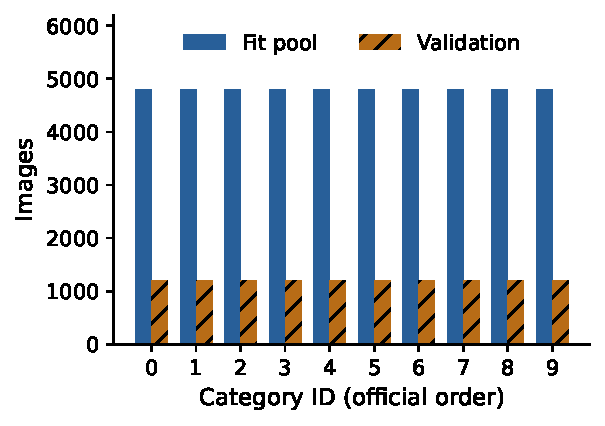
\includegraphics[width=\columnwidth]{figures/class_counts.pdf}
\caption{Class counts in the saved split of official training data. Both pools
are balanced. These are data checks rather than performance measurements.}
\label{fig:counts}
\end{figure}

\section{Features and Models}
\subsection{Fixed Image Representations}
Both paths accept upright raw uint8 images and divide intensities by 255 once.
The pixel path flattens the grid into 784 ordered values. This preserves values
and recoverable positions but supplies no built-in neighborhood or translation
structure to a conventional classifier.

HOG uses 9 orientation bins, 4$\times$4-pixel cells, 2$\times$2-cell blocks and
L2-Hys normalization, with no square-root transform. Seven cells per axis yield
six overlapping blocks per axis, hence
\begin{equation}
d_{HOG}=6\cdot6\cdot2\cdot2\cdot9=1296.
\end{equation}
HOG is therefore a structural representation rather than dimensionality
reduction in this configuration. Its extraction rule is fixed before label-based
training. Figure~\ref{fig:hog} illustrates its edge-direction view.

\begin{figure}[t]
\centering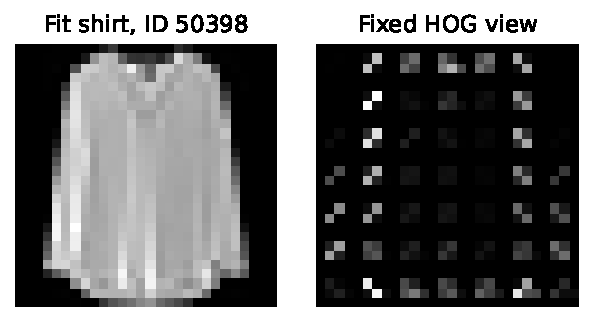
\includegraphics[width=\columnwidth]{figures/hog_example.pdf}
\caption{A fit-partition shirt and its HOG visualization. The visualization
illustrates a fixed descriptor, not learned classifier attention.}
\label{fig:hog}
\end{figure}

StandardScaler is learned inside training Pipelines for Logistic Regression,
SVM and HOG kNN. Pixel kNN and both forest variants use the fixed features
directly. This declared, model-specific choice makes the comparison one of
complete pipelines. Fixed per-image extraction may be cached; learned means
and scales must be fitted only on the fit partition \cite{sklearnpitfalls}.

\subsection{Logistic Regression}
Class scores are $z_c=w_c^Tx+b_c$ and softmax gives
$p(c|x)=\exp(z_c)/\sum_j\exp(z_j)$. Multiclass cross-entropy with regularization
learns the coefficients. Smaller $C$ means stronger regularization. We use
LBFGS with at most 2,000 iterations and validate $C\in\{0.1,1\}$. This is linear
in the supplied representation and need not exploit the same information from
pixels and HOG.

\subsection{k Nearest Neighbors}
kNN stores the fit feature vectors and predicts from a distance-weighted vote
among the nearest examples under Euclidean distance. We validate $k\in\{3,5\}$
with brute-force search. A small fit time is not a low total-compute guarantee:
neighbor search and stored training data make inference and memory important.

\subsection{Random Forest}
We combine 200 bootstrap-trained trees, with square-root feature sampling and
minimum leaf size 1. Gini impurity is $1-\sum_c p_c^2$. Randomization diversifies
trees; depth controls each tree's flexibility. The implementation averages
tree class probabilities. We validate depth 20 versus unrestricted depth,
keeping random seed 42. Tree counts and nodes describe structure, rather than
a directly comparable linear-model parameter count.

\subsection{RBF Support Vector Machine}
The kernel is $K(x,x')=\exp(-\gamma\lVert x-x'\rVert^2)$. $C$ controls the
violation penalty and $\gamma$ the locality of similarity. SVC uses pairwise
classifiers for the ten classes. We validate $C\in\{1,10\}$ and hold
\texttt{gamma='scale'} fixed. Probability estimation is disabled because the
requested metrics need predicted labels. A recorded version-1.9 deprecation
warning concerns that explicit probability option; it is not a convergence
failure. Kernel fitting and support-vector prediction can be costly.

\section{Experimental Protocol}
\subsection{Development and Final Fitting}
The compact search has two candidates for each of eight representation/model
rows, or 16 development fits. Every candidate sees the same stratified 12,000
fit-pool examples and unchanged 12,000 validation examples. A separate
2,000/1,000 smoke path checks the interfaces and cannot unlock final testing.

Within each row, the development candidate with the highest validation macro
F1 is selected, with accuracy, lower validation prediction time and run ID as
tie-breakers. All eight selected configurations are then fitted afresh on the
full 48,000 fit examples. This is not a fit on training plus validation.
The overall model is selected from the eight full-profile validation results
using the same rule. Its ID, all model hashes, settings, split hash and scores
are frozen before loading official test content. Unconverged or failed runs
cannot be selected. Search logs, including the recorded API warning, remain
available.

All final models use identical fit, validation and test IDs. The test results
describe the eight frozen finalists and do not trigger a new selection or
hyperparameter change. The repository stores raw predictions in compressed
CSV files, checks their IDs and true labels, and regenerates metrics in the
executed master notebook.

\subsection{Metrics and Timing}
Accuracy is the correct fraction. For category $c$,
\begin{equation}
R_c=\frac{TP_c}{TP_c+FN_c},\qquad
F1_c=\frac{2TP_c}{2TP_c+FP_c+FN_c}.
\end{equation}
Macro F1 is $\frac{1}{10}\sum_c F1_c$, with labels 0--9 explicitly included and
undefined precision/F1 set to zero. Per-class support accompanies recall.
Rows of a confusion matrix are true classes; row-normalized diagonals equal
recall.

Fit time includes scaler and classifier fitting but excludes fixed feature
extraction and the development search. Inference uses already loaded models
and 1,024 fixed test images in batches of 128, one warmup and five repeats
under one native thread. Pipeline timing starts at cached fixed features.
End-to-end timing includes raw-image normalization, pixel/HOG extraction,
scaler and classifier, excluding disk reads and model loading. We report
median amortized milliseconds per image, not single-request latency.

The recorded environment uses Python 3.12, scikit-learn \LibraryVersion{} and
scikit-image \ImageVersion{} on an Apple ARM64 macOS machine with 16 GiB RAM.
Exact package versions and repeat durations are retained. Absolute timing
depends on hardware, software and concurrent system load.

\section{Results and Error Analysis}
\subsection{Aggregate and Class-Specific Results}
Table~\ref{tab:main} reports the eight full-size final rows. The model selected
before test evaluation, \SelectedName{}, reaches \SelectedAccuracy{} accuracy
and \SelectedFone{} macro F1 on official test data. Figure~\ref{fig:models}
compares the fixed pipelines within classifier families. The separate
most-frequent dummy is a validation reference, not one of the four required
model families.

\begin{table}[t]
\caption{Official test results; all rows fit on the same 48,000 images.
$^*$ marks the overall validation-selected model. Fit time is in seconds.}
\label{tab:main}\centering\small
\begin{tabular}{llrrr}\toprule
Feature & Model & Acc. (\%) & Macro F1 & Fit (s)\\\midrule
Pixels & LR & 84.01 & 0.8394 & 6.9 \\
Pixels & kNN & 85.04 & 0.8505 & 0.0 \\
Pixels & RF & 87.67 & 0.8753 & 57.5 \\
Pixels & RBF SVM & 89.28 & 0.8924 & 100.7 \\
HOG & LR & 87.60 & 0.8757 & 4.2 \\
HOG & kNN & 87.34 & 0.8730 & 0.2 \\
HOG & RF & 87.29 & 0.8718 & 104.9 \\
HOG & RBF SVM$^*$ & 90.91 & 0.9090 & 125.4 \\
\bottomrule\end{tabular}
\end{table}

\begin{figure*}[t]
\centering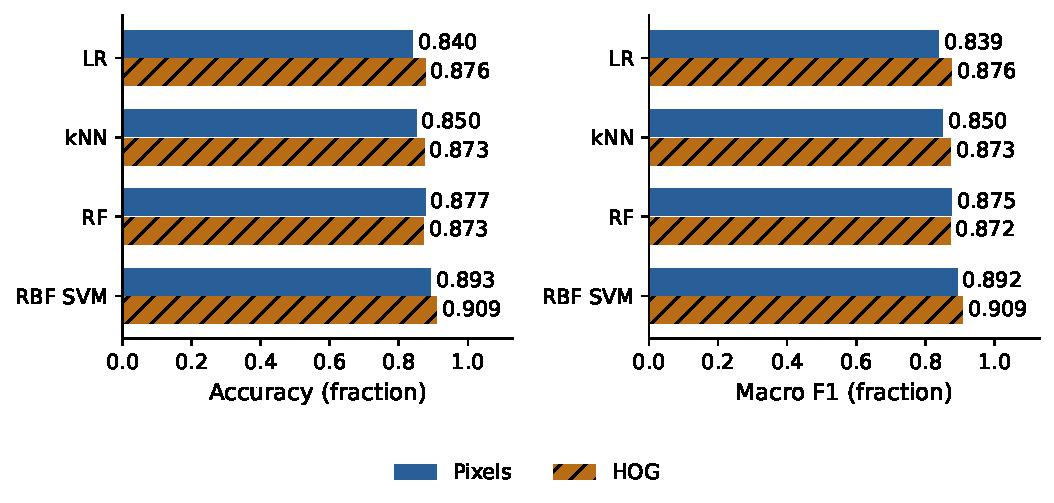
\includegraphics[width=0.97\textwidth]{figures/model_comparison.pdf}
\caption{Pixels versus HOG within each frozen classifier. The comparison changes
the declared representation pipeline; it is not evidence that every possible
HOG/scaler configuration dominates every pixel configuration.}
\label{fig:models}
\end{figure*}

The observed HOG-minus-pixel macro-F1 changes, in percentage points, are
\DeltaText{}. The direction and magnitude should be read within each family,
with the fixed preprocessing and limited tuning budget in mind. These differences
are not claims of statistical significance. Table~\ref{tab:recall} preserves
all ten class recalls instead of hiding weak categories behind aggregate scores.
The validation-selected model's weakest category is \WeakClass{} with
\WeakRecall{} recall.

\begin{table*}[t]
\caption{Test recall in percent for every class; each category has 1,000 actual
test images. T/top means T-shirt/top and Boot means Ankle boot.}
\label{tab:recall}\centering\small\setlength{\tabcolsep}{4pt}
\begin{tabular}{lrrrrrrrrrr}\toprule
Pipeline & T/top & Trouser & Pullover & Dress & Coat & Sandal & Shirt & Sneaker & Bag & Boot\\\midrule
Pixels + LR & 81.1 & 95.6 & 73.0 & 85.8 & 75.2 & 92.5 & 57.2 & 93.0 & 92.5 & 94.2 \\
Pixels + kNN & 83.9 & 96.8 & 79.7 & 85.7 & 76.1 & 80.4 & 60.1 & 95.7 & 95.1 & 96.9 \\
Pixels + RF & 85.7 & 95.7 & 80.1 & 90.6 & 82.3 & 95.5 & 59.4 & 95.0 & 97.5 & 94.9 \\
Pixels + RBF SVM & 84.4 & 97.3 & 82.9 & 89.9 & 82.2 & 96.2 & 69.6 & 96.6 & 97.8 & 95.9 \\
HOG + LR & 83.3 & 97.5 & 79.7 & 87.0 & 81.8 & 95.0 & 66.0 & 94.2 & 97.1 & 94.4 \\
HOG + kNN & 83.5 & 97.5 & 82.3 & 86.6 & 81.6 & 89.0 & 63.7 & 98.1 & 95.4 & 95.7 \\
HOG + RF & 85.1 & 94.8 & 81.2 & 89.4 & 82.2 & 94.8 & 60.2 & 93.7 & 96.8 & 94.7 \\
HOG + RBF SVM & 85.7 & 97.6 & 86.2 & 91.2 & 86.4 & 96.5 & 73.3 & 97.3 & 98.3 & 96.6 \\
\bottomrule\end{tabular}
\end{table*}

\subsection{Observed Confusions and Paired Examples}
For the selected model, the three largest off-diagonal counts are
\ConfusionText{}. Figure~\ref{fig:confusion} focuses on four garment categories;
the complete ten-by-ten count and normalized matrices remain in the notebook
and figure directory. Shared outlines at low resolution are plausible sources
of ambiguity, but the observed mistakes alone do not prove their cause or
that the official labels are wrong.

\begin{figure}[t]
\centering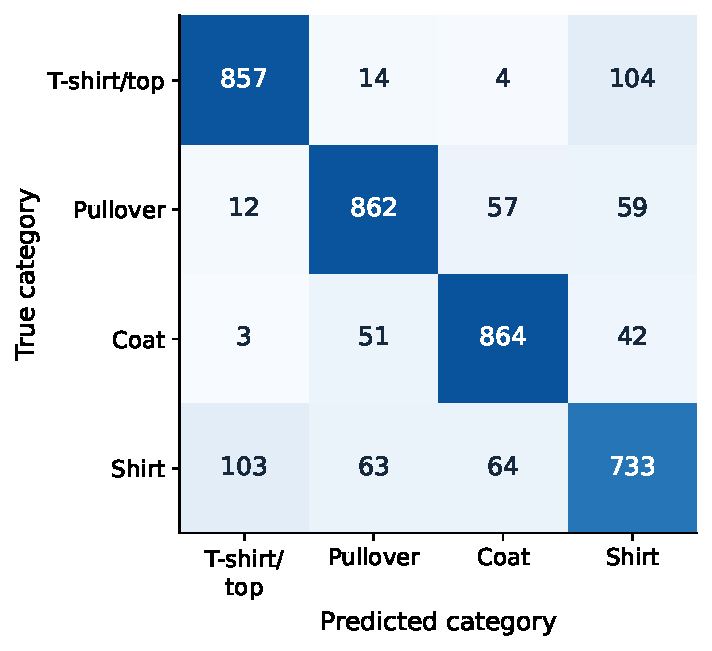
\includegraphics[width=\columnwidth]{figures/focused_confusion.pdf}
\caption{Selected model's test counts for true/predicted T-shirt/top, Pullover,
Coat and Shirt. This is a submatrix, so omitted-category errors are not shown
and displayed rows need not total 1,000. Full matrices are retained separately.}
\label{fig:confusion}
\end{figure}

We align pixel and HOG predictions on identical original IDs within each
classifier, divide images into both-correct, pixels-only-correct,
HOG-only-correct and both-wrong groups, and display the first original IDs in
each group. This rule prevents selectively showing only favorable HOG examples.
Figure~\ref{fig:errors} presents a subset for SVM; complete symmetric panels
and group counts are retained. These post-freeze test examples are descriptive
and were not used to modify the model.

\begin{figure}[t]
\centering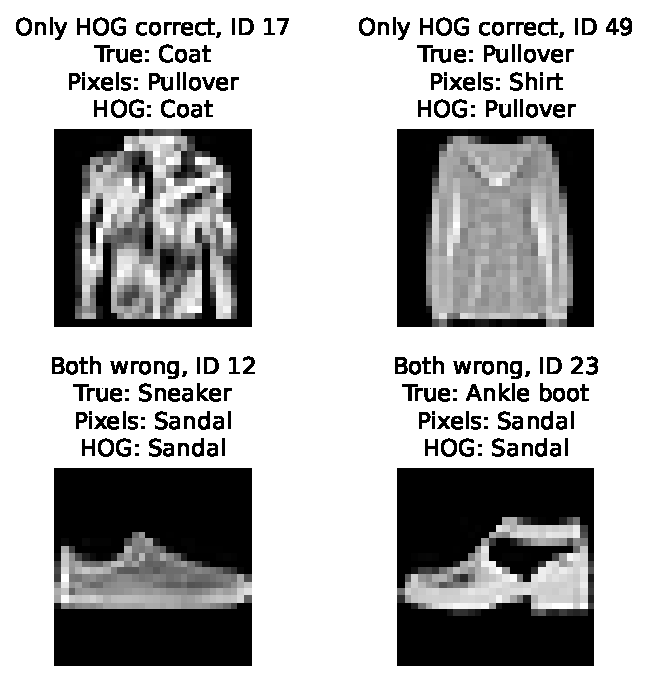
\includegraphics[width=\columnwidth]{figures/error_examples.pdf}
\caption{Paired RBF SVM examples. Each displayed row uses the first two
original test IDs in its outcome group. Additional pixels-only-correct and
both-correct examples are saved with the complete error-analysis artifacts.}
\label{fig:errors}
\end{figure}

\subsection{Inference and Model Storage}
Table~\ref{tab:timing} shows median amortized inference costs and compressed
bundle storage under the same serialization policy. The selected pipeline's
end-to-end measurement is \SelectedLatency{} ms per image. HOG extraction can
change the deployment trade-off even when a classifier predicts quickly.
Search time, training time, model loading and live single-image latency answer
different questions and should not be substituted for this measurement.

\begin{table}[t]
\caption{Inference milliseconds per image, batch-amortized. Storage includes
the compressed model bundle and metadata, in MiB.}
\label{tab:timing}\centering\small
\begin{tabular}{lrrr}\toprule
Pipeline & Predict & End to end & MiB\\\midrule
Pixels + LR & 0.0011 & 0.0014 & 0.05 \\
Pixels + kNN & 0.3291 & 0.3298 & 31.10 \\
Pixels + RF & 0.0758 & 0.0609 & 35.01 \\
Pixels + RBF SVM & 3.2622 & 3.2468 & 39.34 \\
HOG + LR & 0.0014 & 0.1473 & 0.08 \\
HOG + kNN & 0.8365 & 0.9880 & 147.27 \\
HOG + RF & 0.0574 & 0.2061 & 40.24 \\
HOG + RBF SVM & 21.3993 & 21.7090 & 87.82 \\
\bottomrule\end{tabular}
\end{table}

\begin{table}[t]
\caption{Model-specific complexity evidence. Quantities have different meanings
and are not directly interchangeable parameter counts.}
\label{tab:complexity}\centering\small
\begin{tabular}{llr}\toprule
Pipeline & Type & Count\\\midrule
Pixels + LR & W & 7,850 \\
Pixels + kNN & X & 37,632,000 \\
Pixels + RF & N & 1,633,648 \\
Pixels + RBF SVM & S & 13,725,289 \\
HOG + LR & W & 12,970 \\
HOG + kNN & X & 62,208,000 \\
HOG + RF & N & 1,828,070 \\
HOG + RBF SVM & S & 27,295,425 \\
\bottomrule\end{tabular}
\end{table}

Table~\ref{tab:complexity} uses W for learned classifier coefficients plus
intercepts, X for stored kNN training-feature scalars, N for total forest nodes,
and S for SVC support-vector, dual-coefficient and intercept array scalars.
kNN has no learned coefficient count; this is recorded as not applicable rather
than computationally free. Scaler mean/scale counts are stored separately.
Storage also depends on data type, compression and implementation details.

\section{Limitations and Phase 2 Plan}
The results use a single fixed split, one seed, two candidates per row and one
HOG configuration. They do not establish globally optimal hyperparameters,
statistically significant differences, or robustness to domain shift. The
benchmark excludes much of the variation in production catalogue photographs.
Exact duplicate checks are narrower than a semantic or near-duplicate audit.
The representation comparison includes the disclosed scaler policy.

In Phase 2, a small two- or three-block CNN can test whether task-learned local
features improve the remaining category confusions. That experiment should
reuse the saved fit/validation/test membership, select architecture and early
stopping using training-derived validation data, and compare accuracy, macro
F1, recall and documented inference cost fairly. Since Phase 1 already reveals
test outcomes, architecture choices must not be tuned to those outcomes.
Any claimed hybrid method requires a meaningful technical rationale and its
own evidence; no hybrid improvement is claimed here.

\section{Reproducibility and Contributions}
The repository at \url{https://github.com/Nakul-Jaglan/aml-dl-t089} contains
source modules, meaningful integrity tests, saved split IDs, checksums,
validation candidate logs, a hashed freeze manifest, ID-aligned predictions,
metrics, figures and an executed master notebook. A fresh reproduction writes
to an isolated output directory so checked-in frozen evidence stays intact.
Large trained bundles, raw downloads and feature caches are regenerated locally
instead of committed to Git.

Team responsibilities cover integration, literature and report assembly
(Nakul), data quality and EDA (Sudeshhna), visual features, LR and kNN (Puneet),
RF, SVM and experiment management (Samarth), and evaluation and error analysis
(Neelanshu). The repository's contribution record tracks preparation and
individual reviews. Each presenter should be able to explain the shared
pipeline in the individual viva. Section A is confirmed. Student identifiers
appear only in the private submission copy. Institutional affiliation details
and faculty-specific formatting requirements require team confirmation.

\section{Conclusion}
The controlled Phase 1 experiment compares eight classical pipelines under
shared data membership and validation-only model selection. The selected
\SelectedName{} achieves \SelectedAccuracy{} official-test accuracy and
\SelectedFone{} macro F1. Per-class recalls, paired errors and measured compute
costs qualify the aggregate result. HOG's contribution is empirical and
classifier-dependent under the declared preprocessing policy. Learned spatial
features remain a concrete question for Phase 2 rather than a result asserted
in advance.

\bibliographystyle{IEEEtran}
\bibliography{references}
\end{document}
